\documentclass[11pt]{article}

\usepackage[margin=1in]{geometry}
\usepackage{fancyhdr}
\pagestyle{fancy}
\usepackage{hyperref} %for hyperlinks
\usepackage{gensymb} %for symbols such as \degree
\usepackage{amsmath}
\usepackage{amssymb}
\usepackage{graphicx}
\usepackage{float} %for graphics placement

\lhead{Hannah Holland-Moritz}
\chead{Zen DNA Extraction Protocol}
\rhead{\today}


\begin{document}

\begin{center}
\textbf{\large{Zen DNA Extraction Protocol}}
\break

\emph{This protocol is a modified version of the \href{http://www.mobio.com/images/custom/file/protocol/12888.pdf}{MoBio PowerSoil\textsuperscript{\tiny{ \textregistered   }}DNA Isolation Kit} protocol.} The modifications are for time-saving and Zen-specific extraction optimization.
\end{center}

\textbf{Before starting:} 
\begin{itemize}
\item
Set heat block to 60\degree C
\end{itemize}
\hfill
\hfill
\begin{enumerate}
\item
After following the \textbf{Zen Pre-Extraction protocol}, all samples should be in \textbf{PowerBead} tubes.

\item 
\textbf{Check Solution C1}. If \textbf{Solution C1} is precipitated, heat solution to 60\degree C until dissolved before use.

\item
Add 60 $\mu$l of \textbf{Solution C1} and vortex briefly. \emph{Note: You will see a white precipitate formed as a result of the cold temperature of the tubes and C1 mixing with the Zymo Stabilization buffer.}


\item
Place \textbf{PowerBead tubes} in heat block at 60\degree C for 5 minutes.

\item 
Place \textbf{PowerBead tubes} in bead-beater for 2-3 minutes.

\item
While bead-beating, prepare \textbf{2ml Collection tubes}: Add 250 $\mu$l of \textbf{Solution C2} to each.

\item
Make sure the \textbf{PowerBead Tubes} rotate freely in your centrifuge without rubbing. Centrifuge tubes at 10,000 x g for 1 minute at room temperature. \textbf{CAUTION:} Be sure not to exceed 10,000 x g or tubes may break.

\item 
Transfer 420 $\mu$l of the supernatant to \textbf{2 ml Collection Tub}e with C2.
\emph {Note: Expect between 400 to 500 of supernatant. Left-over supernatent may be stored at -20\degree C for later extraction. Supernatant may still contain some soil particles.}

\item 
Vortex for 5 seconds. Incubate at 4\degree C for 5 minutes.

\item 
While C2 tubes are incubating, prepare \textbf{2ml Collection tubes}: Add 200 $\mu$l of \textbf{Solution C3} to each.

\item
Centrifuge the tubes containing C2 at room temperature for 1 minute at 10,000 x g.

\item
Avoiding the pellet, transfer up to, but no more than, 600 $\mu$l of supernatant to a C3-filled \textbf{2 ml Collection Tube}.

\item
Vortex C3 tubes for 5 seconds. Incubate at 4\degree C for 5 minutes.

\item
While C3 tubes are incubating, prepare \textbf{2ml Collection tubes} and \textbf{Spin Filters}: 	\begin{itemize}
	\item
	Organize open \textbf{2ml Collection tubes} and open \textbf{Spin Filters} opposite each other on a rack. (See diagram)
	\item
	Shake to mix \textbf{Solution C4} before use. Add 1200 $\mu$l of \textbf{Solution C4} to the \textbf{2ml Collection tubes}. 
	
	\emph{Note: This may take longer than 5 minutes to accomplish. If so, remove incubating tubes and finish task while centrifuging.}
	\end{itemize}

\begin{figure}[H] %image placed exactly where it is in code
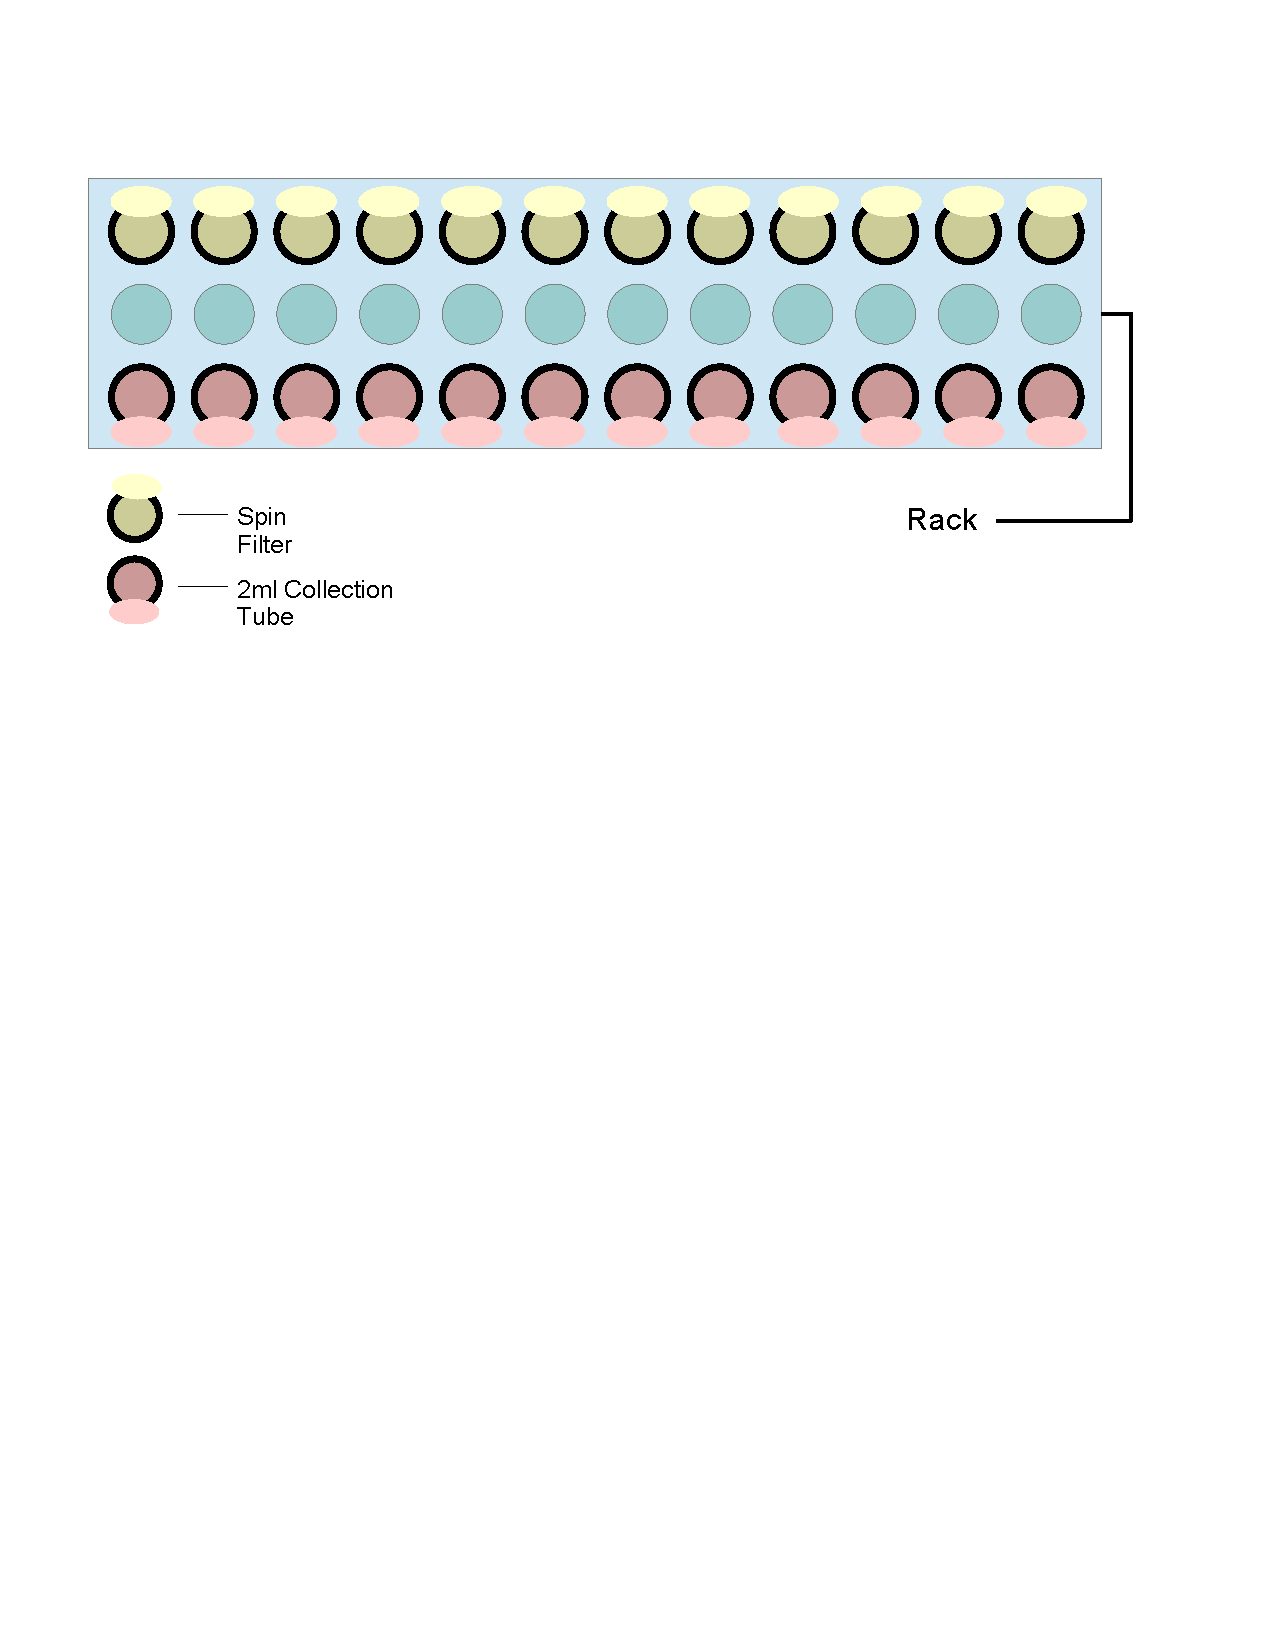
\includegraphics[scale=0.9, trim = 10mm 170mm 20mm 30mm, clip]{Extraction_diagram.pdf}
\caption{Collection tube and Spin Filter arrangement.}
\end{figure}
	
\item
Centrifuge the tubes containing C3 at room temperature for 1 minute at 10,000 x g.

\item
Set pipette to 800 $\mu$l. Carefully avoiding the pellet remove \textbf{all supernatant} from tube. In C4-filled \textbf{2ml Collection tube} carefully pipette up and down 4-8 times to mix, then fill open \textbf{Spin Filter} with mixed liquid. Dispense remaining liquid back into the 2ml Collection tube and \emph{carefully} eject pipette tip into open 2ml Collection tube.

\emph{Note: Avoid over-filling spin filter or it will over-flow when capped. If working with a pipette which violently ejects tips, discard tip in trash instead of ejecting into 2ml Collection tube.}

\item
Centrifuge \textbf{Spin Filters} at 10,000 x g for 1 minute at room temperature. Discard flow through and refill with C4-supernatant mixture using previous pipette tips. Repeat 3 times or until C4-supernatant mix is used up.

\item
Add 500 $\mu$l of \textbf{Solution C5} and centrifuge at room temperature for 1 minute at 10,000 x g. Discard the flow through.

\item
Centrifuge again at room temperature for 1 minute at 10,000 x g.

\item
While centrifuging, prepare \textbf{2ml Collection tubes} to receive spin filters.

\item
Carefully place spin filter in clean \textbf{2 ml Collection Tubes}. Avoid splashing any \textbf{Solution C5} onto the \textbf{Spin Filter}.

\item
Add 100 $\mu$l of \textbf{sterile DNA-Free PCR Grade Water} to the center of the white filter membrane.

\item
Centrifuge at room temperature for 1 minute at 10,000 x g.

\item
Discard the Spin Filter. The DNA in the tube is now ready for any downstream application. No further steps are required. Store between -20\degree to -80\degree C.

\end{enumerate}

\end{document}
